%% Template for ENG 401 reports
%% by Robin Turner
%% Adapted from the IEEE peer review template

%
% note that the "draftcls" or "draftclsnofoot", not "draft", option
% should be used if it is desired that the figures are to be displayed in
% draft mode.

\documentclass{article}
\usepackage{url} % Provides better formatting of URLs.
\usepackage[utf8]{inputenc} % Allows Spanish characters.
\usepackage[spanish]{babel}
\usepackage{amssymb}
\usepackage{booktabs} % Allows the use of \toprule, \midrule and \bottomrule in tables for horizontal lines
\usepackage{float}
\usepackage{pdfpages}
\usepackage{graphicx}
\usepackage{booktabs}
\usepackage{fancyhdr}
\usepackage{eurosym}
\usepackage{calendar}



\hyphenation{op-tical net-works semi-conduc-tor} % Corrects some bad hyphenation 



\begin{document}
%\begin{titlepage}
% paper title
% can use linebreaks \\ within to get better formatting as desired
\title{
\includegraphics[scale=0.65]{logoDefinitivo1.png} \\ \textbf{Proyecto UPBEAT} \\ \textbf{Grupo 03. Barbara Liskov}\\Plan de gestión, análisis y memoria del proyecto \vspace{0.1cm} \\}

% author names and affiliations

\author{Alejandro Ruiz Sumelzo\\
Alejandro Piedrafita Barrantes\\
Álvaro Santamaría De la Fuente\\
Fernando Navarro Zarralanga\\
José Félix Yagüe Royo\\
Víctor Pérez Sanmartín\\
Sergio Torres Castillo \vspace{0.25cm}
\\\\

\includegraphics[scale=0.5]{logoUZ.png}\\
}
\date{16 de marzo de 2020}

% make the title area
\maketitle
\newpage
\section*{Introducción}
El proyecto \textit{Upbeat} consiste en el desarrollo e implementación de un reproductor de música en streaming.\\
\hfill \break
La aplicación está diseñada para todo tipo de público, incluidos artistas. Permitirá a los usuarios escuchar canciones o podcasts, crear listas de reproducción, añadir canciones o podcasts a su lista de favoritos para después acceder a sus contenidos preferidos de una forma más rápida o seguir a otros usuarios entre otras funcionalidades.
\hfill \break\\
De manera similar, los artistas tendrán las mismas características que cualquier usuario además de poder subir canciones y/o crear álbumes. Esto será algo exclusivo de las cuentas de clientes registradas como artistas.
\hfill \break
Añadirá aspectos de la 'red social', tales como seguir a otros usuarios o sus playlist creadas.\\
\hfill \break
Otras de las características diferenciales de nuestra aplicación será el uso de banners de publicidad o la implementación de un ecualizador de sonido que modificará la manera de reproducir las canciones.\\\\
Por último, el reproductor de música \textit{Upbeat} permitirá realizar una búsqueda por título de canción, género, artista y país de la misma.\\\\
Se permitirá usar la aplicación de tres maneras diferentes: Mediante una aplicación web (navegador Chrome), una aplicación para dispositivos\textit{Android} y una aplicación para dispositivos \textit{iOS}.\\\\
Las 3 versiones de la aplicación serán muy similares, salvo que un pequeño número de características solo estarán disponibles en la versión web, como el ecualizador de sonido o los banners de publicidad. \\\\
Usará también un sistema de sincronización, permitiendo que el usuario retome cualquier canción donde la había dejado, en todos los dispositivos.


\newpage
\tableofcontents % si estas líneas se comentan, se eliminan los índices
%\listoffigures
%\listoftables
\addtocontents{toc}{\hfill \textbf{Página} \par}
\newpage
\pagestyle{fancy}
\lhead{\begin{picture}(0,0) \put(0,0){\includegraphics[width=40mm]{logoEina.png}} \end{picture}}
\rhead{\begin{picture}(0,0) \put(-100.7,0){
\includegraphics[width=35mm]{logoDefinitivo3.png}} \end{picture}}
\section{Organización del proyecto}
\begin{table}[H]
	\hspace*{-3.7cm}
	\centering
	\begin{tabular}{|l|l|l|}
		\hline
		\multicolumn{1}{|c|}{\textbf{Integrante}} & \multicolumn{1}{c|}{\textbf{Puesto}} & \multicolumn{1}{c|}{\textbf{Responsabilidades}}\\ \hline
		Alejandro Ruiz Sumelzo                    & \begin{tabular}[c]{@{}l@{}}Director del proyecto.\\ Coordinador y desarrollador del grupo de back-end.\\ Encargado de la documentación del análisis y diseño\\ del sistema.\end{tabular} & \begin{tabular}[c]{@{}l@{}}Responsable de redactar algunas actas\\ en reuniones con el profesor.\\ Control de la distribución de trabajo\\ (elaboración de calendario) y \\ revisión de esfuerzos.\\ Desarrollador de modelos, repositorios y \\controladores de la API.\\ Encargado del despliegue del back end \\sobre el servidor.\end{tabular} \\ \hline
		\begin{tabular}[c]{@{}c@{}}Alejandro\\ Piedrafita Barrantes\end{tabular}
		&                                                                       Desarrollador de apoyo para el grupo de back-end                                                                                                                 &  
		\begin{tabular}[c]{@{}l@{}}Realización de tareas de gestión\\  (edición de memoria y otros documentos).\\ Desarrollador de modelos, repositorios y \\ controladores de la API. \\ Diseño del sistema mediante diagramas.\end{tabular}\\ \hline
		\begin{tabular}[c]{@{}c@{}}Víctor\\ Pérez Sanmartín\end{tabular}
		&                                                                       Desarrollador de apoyo para el grupo de back-end                                                                                                                 &  
		\begin{tabular}[c]{@{}l@{}}
		Responsable de redactar algunas actas\\ en reuniones con el profesor.\\
		Realización de tareas de gestión\\  (edición de memoria y otros documentos).\\ Desarrollador de modelos, repositorios y \\ controladores de la API. \\ Encargado del diseño e implementación\\ de la base de datos.\end{tabular}\\ \hline
		\begin{tabular}[c]{@{}c@{}}Álvaro Santamaría\\ de la Fuente\end{tabular}
		& \begin{tabular}[c]{@{}l@{}}  Desarrollador del grupo de front-end móvil.\end{tabular}     &  
		\begin{tabular}[c]{@{}l@{}}
		Realización de tareas de gestión\\ (edición de memoria y otros documentos).\\
		Desarrollo e implementación del front-end \\de la aplicación móvil.\\
		Implementar la lógica de la aplicación de\\ \textit{Android} e \textit{iOS}.\\
		Encargado de unificar las partes \\de la aplicación móvil y llevar a cabo \\ el despliegue en \textit{Android} e \textit{iOS}.
		\end{tabular}\\ \hline
		\begin{tabular}[c]{@{}c@{}}José Félix Yagüe\\ Royo\end{tabular}
		&                                                                       \begin{tabular}[c]{@{}l@{}}  Desarrollador del grupo de front-end móvil.\\ Encargado de la gestión de la parte front móvil \\ del proyecto.\end{tabular}                                                  &  
		\begin{tabular}[c]{@{}l@{}}Realización de tareas de gestión\\ (edición de memoria y otros documentos).\\
		Desarrollo e implementación del front end \\de la aplicación móvil.\\
		Encargado de la conexión con el API REST. \\
		Control de la distribución de trabajo y \\ coordinación dentro del grupo \\ front-end de móvil.\\\end{tabular}\\ \hline
	\end{tabular}
\end{table}

\begin{table}[H]
	\hspace*{-3.7cm}
	\centering
	\begin{tabular}{|l|l|l|}
		\hline
		\multicolumn{1}{|c|}{\textbf{Integrante}} & \multicolumn{1}{c|}{\textbf{Puesto}} & \multicolumn{1}{c|}{\textbf{Responsabilidades}}\\ \hline
		\begin{tabular}[c]{@{}c@{}}Fernando\\ Navarro Zarralanga\end{tabular}           
		& 
		\begin{tabular}[c]{@{}l@{}}Coordinador y desarrollador del grupo de \\ front-end web.\\ Encargado de la gestión de la parte front web \\ del proyecto.\end{tabular} & \begin{tabular}[c]{@{}l@{}}Realización de tareas de gestión\\ (edición de memoria y otros documentos).\\ Diseñar pantallas de la aplicación de la web.\\
		Implementar la lógica de la \\ aplicación web.\\ 
		Encargado de llevar a cabo el despliegue \\de la web.
		\end{tabular} \\ \hline
		\begin{tabular}[c]{@{}c@{}}Sergio\\ Torres Castillo\end{tabular}
		&                                                                       Desarrollador de apoyo para el grupo de front-end                                                                                                                 &  
		\begin{tabular}[c]{@{}l@{}}
			Realización de tareas de gestión\\ (edición de memoria y otros documentos).\\
			Diseñar pantallas de la aplicación de la web.\\ Implementar parte de la lógica de la \\aplicación web.\end{tabular}\\ \hline
	\end{tabular}
\end{table}
\newpage
\section{Plan de gestión del proyecto}

\subsection{Procesos}

\subsubsection{Procesos de inicio del proyecto}
En el equipo de front-end de movil se va a utilizar \textit{Android Studio} como entorno de desarrollo, y \textit{Flutter} como \textit{SDK}, el cual utiliza \textit{Dart} como lenguaje de programación. Para la realización de las pruebas, se van a utilizar tanto un emulador, como un móvil real con \textit{Android 10}. Para \textit{iOS} se va a instalar \textit{XCode} en \textit{Mac} ya que es el IDE oficial de \textit{Apple}, pero se va a mantener tanto \textit{Flutter} como \textit{Dart} para su desarrollo, y un emulador para las pruebas. La aplicación requerirá tener instalado \textit{Android} 5.0 mínimo para funcionar.\\
\hfill \break
De manera similar, para la realización de la aplicación web, solamente es necesario tener \textit{Google Chrome} para hacerlo funcionar. El desarrollo se realizará sobre \textit{VSCode}.
\hfill \break
Se ha elegido un tamaño de 500 MB en la BD, suficiente para llevar a cabo pruebas con diversas canciones y configuraciones.\\
\hfill \break
En la realización del proyecto se ha compilado y ejecutado toda la parte de back-end sobre un portátil \textit{MSI} con la siguientes características:
\begin{itemize}
	\item Windows 10 Pro
	\item Latest 6th Gen. Intel® Core™ i7 processor
	\item NVIDIA® GeForce GTX 960M
	\item 15.6" Full HD (1920x1080)
	\item NVMe M.2 SSD by PCIe Gen3 X4
	\item USB 3.0 Type-C reversible plug
	\item 8 GB RAM
\end{itemize}
En la realización del proyecto se ha compilado y ejecutado la parte de front-end móvil sobre un portátil \textit{Lenovo} con la siguientes características:
\begin{itemize}
	\item Windows 10 Pro
	\item Latest 5th Gen. Intel® Core™ i5 processor
	\item 15.6" Full HD (1920x1080)
	\item 120 GB SSD
	\item 4 GB RAM
\end{itemize}
En la realización del proyecto se ha compilado y ejecutado la parte de front-end aplicación web sobre un portátil \textit{Acer} con la siguientes características:
\begin{itemize}
	\item Windows 10 Home
	\item Latest 7th Gen. Intel® Core™ i3 processor
	\item 15.6" Full HD (1920x1080)
	\item 240 GB SSD
	\item 8 GB RAM
\end{itemize}

\subsubsection{Procesos de ejecución y control del proyecto}
Las comunicaciones internas se llevarán a cabo mediante un grupo de \textit{WhatsApp} estimado para ello, para cualquier otra duda o comunicación entre componentes del equipo se hará de forma individual. La resolución de tareas será totalmente independiente y completa en el entorno de \textit{GitHub}.\\
\hfill \break
Los responsables de realizar la puesta en marcha serán los encargados de la parte front-end y de la parte back-end. La creación de copias de seguridad y semejantes se realizarían de manera automática gracias a \textit{GitHub}. 
\hfill \break
El repositorio que se creará con todos los archivos referentes al proyecto se encontrará en \textit{GitHub}, para que todos los integrantes del proyecto puedan acceder fácilmente a los archivos. Además, se usará el \textit{Issue Tracker} de \textit{GitHub} para la gestión de incidencias; el director del mismo se encargará de crear las incidencias principales, y cada uno de los encargados de cada parte las completarán en cada uno de sus ámbitos.\\
\hfill \break
El proyecto estará dividido en varios repositorios: uno específico para front-end, otro para back-end, y la memoria. Para conseguir que no se modifique el mismo fichero por dos personas al mismo tiempo y evitar problemas, cada equipo tendrá más subramas de desarrollo, por ejemplo, una para cada miembro del equipo, que serán actualizadas con cambios no siempre funcionales y cuando sean más estables se volcarán a la rama de desarrollo principal. 
\hfill \break
En la rama principal de cada uno de los repositorios, sólo podrá haber una versión funcional del sistema, que antes de ser subida será sometida a diferentes test automáticos, entre los que se incluirán test para comprobar la estabilidad del sistema (pruebas de sobrecarga) y test que revisarán las acciones disponibles para comprobar los requisitos que se han resuelto, además de ser testeado por varios miembros del equipo. 
\hfill \break
Para que lo desarrollado en cada uno de estos repositorios pase al repositorio funcional, cada líder de las respectivas partes revisará el código actualizado y si todo está correcto se considerará válido. \\
\hfill \break
Durante el desarrollo del proyecto puede haber problemas y disputas entre los miembros del equipo. Para tratar de resolverlos los coordinadores serán los primeros en mediar entre los miembros en disputa y, si hay alguna razón que haga imposible esta mediación, será el resto del equipo quien deberá votar en consecuencia. 
\hfill \break
Todos los componentes del equipo son capaces de modificar los ficheros de los repositorios, excepto en el de las versiones, el cual solo podrán subir archivos y modificarlos los líderes del front-end y el back-end.

\subsubsection{Procesos técnicos}
En primer lugar, en el front-end web se ha utilizado la herramienta \textit{Angular} que utiliza \textit{JavaScript}, \textit{HTML} y \textit{CSS}. Se han utilizado librerías ya predefinidas en la guía de estilo \textit{Angular Material} para los elementos de diseño, como por ejemplo \textit{MatForms}, \textit{MatIcons} y \textit{HttpClient}. Para desplegar y probar la aplicación hemos empleado el navegador \textit{Google Chrome}.
Para usar esta herramienta ha sido necesario utilizar el manual de \textit{Angular} y algunos tutoriales online de \textit{JavaScript} y \textit{CSS}.\\
\hfill \break
Para el desarrollo del software de la parte del Front-end de la aplicación móvil se va a utilizar el entorno de \textit{Android Studio} haciendo uso de su integración con \textit{git} para facilitar el control de versiones y así, gestionar de forma uniforme entre los dos integrantes del grupo, el repositorio \textit{Flutter} en el que se irá desarrollando el software correspondiente a la aplicación móvil. Para las pruebas en el dispositivo de \textit{iOS} se utilizará el entorno de \textit{VSCode}.\\\\
Para el proceso de prueba de funcionalidades de la aplicación móvil se seguirá el siguiente guión:
	\begin{itemize}
		\item Primero el desarrollador se asegurará de tener la última versión del repositorio \textit{Flutter}, efectuando un pull de la rama que desea testear.
		
		\item A continuación se abre el entorno de desarrollo (VSCode en caso de que se vaya a probar la aplicación en iOS o Android Studio en el caso de un dispositivo Android) y se procede a buildear el código de la app. En caso de encontrar errores se notificarán al encargado de haber realizado esa parte del código.
		
		\item Se ejecuta la aplicación libre de errores de compilación en el dispositivo deseado (iOS o Android)
		
		\item Posteriormente se realiza la prueba de la nueva funcionalidad implementada, comprobando que no se dan situaciones de error ni resultados inesperados.
		
		\item Si las pruebas realizados han sido satisfactorias, se informará al coordinador del grupo de front-end móvil y realizará un merge de esa rama con la rama máster.
		
		\item Las versiones utilizadas en los entornos de desarrollo han sido:
		\begin{itemize}
			\item \textit{Flutter}: v1.12.13 + \textit{hotfix} .9
			\item \textit{Android SDK}: v29.0.3
			\item \textit{Android Studio}: v3.6
			\item \textit{Angular}: v9.0
			\item \textit{Node JS}: v12.16.2 LTS
		\end{itemize}
	\end{itemize}
\newpage
\subsection{Planes}

\subsubsection{Plan de gestión de configuraciones}
La convención de nombres utilizadas para nombrar los distintos archivos sería la siguiente: 
\begin{figure}[H]
	\centering{
		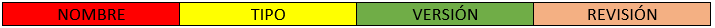
\includegraphics[scale=0.55]{conf1.png}}
\end{figure}
Las versiones solo se modificarán cada vez que se produzcan cambios suficientemente importantes, como por ejemplo la implementación de una nueva funcionalidad. 
Cada vez que se cree una nueva versión, pero sus cambios sean menores, como resolución de errores, se modificará su número de revisión, pero no de versión. 
Se crearán ficheros de documentación que permita ir recopilando toda la información referente a los cambios.\\
\hfill \break
Además, en los ficheros de documentación en los que se expliquen las diversas funcionalidades que tiene la aplicación y que errores se han ido resolviendo, cuando estos sean de una nueva versión o revisión solo se ofrecerá la información sobre los cambios que existan entre esta y la versión o revisión anterior, pero siempre que se cambie la versión se documentarán los cambios respecto a la primera revisión de la versión anterior (p.ej. La versión 2.1 solo contendrá las novedades respecto a la versión 2.0, pero la versión 3.0 contendrá todos los cambios que hayan sucedido desde la versión 2.0 aunque la mayoría se hayan documentado ya en las revisiones).\\
\hfill \break
Todas las semanas habrá una serie de tareas asociadas mediante el \textit{Issue Tracker}. Al final de cada semana, el responsable de cada parte del proyecto revisa las tareas que se han realizado esa semana y se realiza un seguimiento de las mismas: si hay tareas que no se han cumplido, se asigna automáticamente para la siguiente semana, siendo estas tareas las primeras que se deberán hacer.  
\hfill \break
Además, cada semana el responsable de cada una de las partes revisará cuántas tareas se han realizado para la siguiente iteración, controlando si han sido completadas o no y cuánto tiempo de retraso acumula respecto a la planificación original.  Tras esta revisión, este responsable asignará las tareas de la semana a todos los miembros del equipo que puedan trabajar esa semana. \\
\hfill \break
Por último, la distribución del proyecto en el \textit{GitHub} son cuatro carpetas:
\begin{itemize}
	\item UNIZAR-30226-2020-03/Memoria
	\item UNIZAR-30226-2020-03/Angular-Front
	\item UNIZAR-30226-2020-03/Spring-back
	\item UNIZAR-30226-2020-03/Flutter
\end{itemize}

\newpage
\subsubsection{Plan de construcción y despliegue del software}
Respecto a la parte front-end web, la manera utiliza para desplegar el software para probarlo se ejecuta mediante la línea de comandos y un servidor virtual accesible desde un navegador local (como \textit{Chrome}) mediante la ruta \textit{localhost} y el puerto \textit{4200}. No se requiere ningún tipo de autentificación para ello.
Algo a destacar es la omisión por parte de \textit{GitHub} de la carpeta de módulos de Angular (librerías que utiliza el proyecto), ya que ocupa demasiado, de tal forma que cada uno tiene que tener su propia carpeta de librerías.\\
\hfill \break
Para la parte móvil, el uso de \textit{Android Studio} y \textit{Gradle} permite la instalación automática de las dependencias necesarias del proyecto, además de compilar el mismo cada vez que se prueba una parte del código.\\
\hfill \break
Para comprobar cada una de las funcionalidades que se van añadiendo, se realizan de manera manual, primero en los ordenadores personales de cada integrante y luego integrándolo con el servidor de producción. 
Los módulos son independientes entre ellos y se comunican principalmente mediante peticiones \textit{HTTP}, esto permite simular las peticiones antes de probarlo con el entorno real de producción. 
Este servidor de producción es \textit{Heroku}. \\
\hfill \break
En la parte referente al back-end, la construcción y despliegue se realizan de la siguiente manera:
\begin{enumerate}
	\item Se lanza la base de datos \textit{upbeat} de \textit{PostgreSQL} con usuario: \textit{ekngbyjaefrukg} y contraseña: \textit{805e38675224c7f5e8d95d472af06a341b6e3f1de59980b2\\6eae0b16b22eb4a6} en el puerto \textit{5432}.
	\item Esto se debe a que la aplicación se despliega automáticamente en Heroku.
	\item Establecer puerto en las propiedades del proyecto \textit{Spring} para las conexiones \textit{HTTP} (por defecto se usará el \textit{8080} pero podría llegar a cambiarse en caso de puertos ya ocupados/escuchando).
	\item Compilar el proyecto utilizando \textit{Maven}, el cual facilita las dependencias de nuestro proyecto asegurándose que todo quede compilado con las mismas dependencias y funcione correctamente.
	\item Lanzar el proyecto de \textit{Spring} (\textit{Run})*.
	\item Para la comprobación del correcto funcionamiento de la parte referente al back-end, antes de conectar con los respectivos proyectos de \textit{Angular} y \textit{Flutter} (front-end) se utilizará la aplicación \textit{Postman}. Esta herramienta nos permite hacer peticiones \textit{GET} y \textit{POST} y poder observar su resultado.
	\item En el momento que se produce una subida a la rama master, se despliega automáticamente en \textit{Heroku}, por lo que las parte front-end puede hacer peticiones sin tener que correr este back-end en local.
\end{enumerate}


\subsubsection{Plan de aseguramiento de la calidad}
Para asegurar la calidad, en el caso de la aplicación \textit{Android} se usará la guía de estilo de \textit{Android} \footnote{https://developer.android.com/design}, siguiendo algunos consejos que ahí se comentan, siguiendo los principios de utilización de color principal, siendo este el azul cian, legibilidad y jerarquía, con el objetivo de facilitar la compresión del usuario sobre la interfaz con elementos intuitivos y fácilmente reconocibles. \\
En la aplicación web, se usará determinados ejemplos de la página de \textit{Angular} \footnote{https://angular.io/} creada por \textit{Google}, la cual permite usar y conocer conceptos importantes a la hora de hacer un código limpio y eficiente.\\
En ambas guías se sigue el consejo de usar 80 carácteres por línea.
\hfill \break
Además, siempre se realizarán las pruebas necesarias antes de realizar un \textit{commit} con la última actualización del proyecto validado. Por lo que la versión que residirá en \textit{GitHub} será la correcta. 
\hfill \break
Una vez que la base de datos, aplicación web y móvil, estén terminadas y funcionen con el servidor, se seguirán unas determinadas pautas para comprobar que la aplicación funciona correctamente en todos ellos.  
Unido a todo esto, es imprescindible el uso de ambas aplicaciones por personas ajenas al proyecto, recogiendo opiniones sobre la usabilidad del sistema y detectar posibles errores. 

\subsubsection{Calendario del proyecto y división del trabajo}
En la primera iteración del proceso de diseño nos centraremos en desarrollar las funcionalidades principales del sistema, mientras que en la segunda iteración se corregirán todos los errores encontrados en la primera, se implementarán las funcionalidades secundarias y se afinara el diseño de la página web y de las aplicaciones móviles para que sean más agradables al usuario. 
\hfill \break
Para la primera iteración, se planea permitir la creación, edición y borrado de clientes con sus credenciales básicos: nombre de usuario, nombre real, correo, contraseña. Unido a esto, comprobar si las entidades Artista y Usuario se crean y borrar correctamente.  También se permitirá la subida de canciones por parte de los artistas; estas canciones serán visibles en la aplicación y podrán ser reproducidas (al igual que los podcasts). Los álbumes estarán disponibles con su descripción y podrán ser consultados, reproduciendo cada una de sus canciones.
\hfill \break
Para la segunda iteración se finalizarán los requisitos que, por falta de tiempo, no pudieron ser completados en la primera y se añadirán funcionalidades al sistema. Estas funcionalidades son: añadir canciones a la lista de reproducción de un usuario, permitir información adicional en los perfiles de usuario (como puede ser una foto de perfil, una descripción, etc.), además de poder seguirse entre dos usuarios. Se permitirá la búsqueda y filtrado de determinadas canciones y/o álbumes por unos determinados parámetros, al igual que utilizar un ecualizador en la aplicación web con el uso de \textit{banners}.

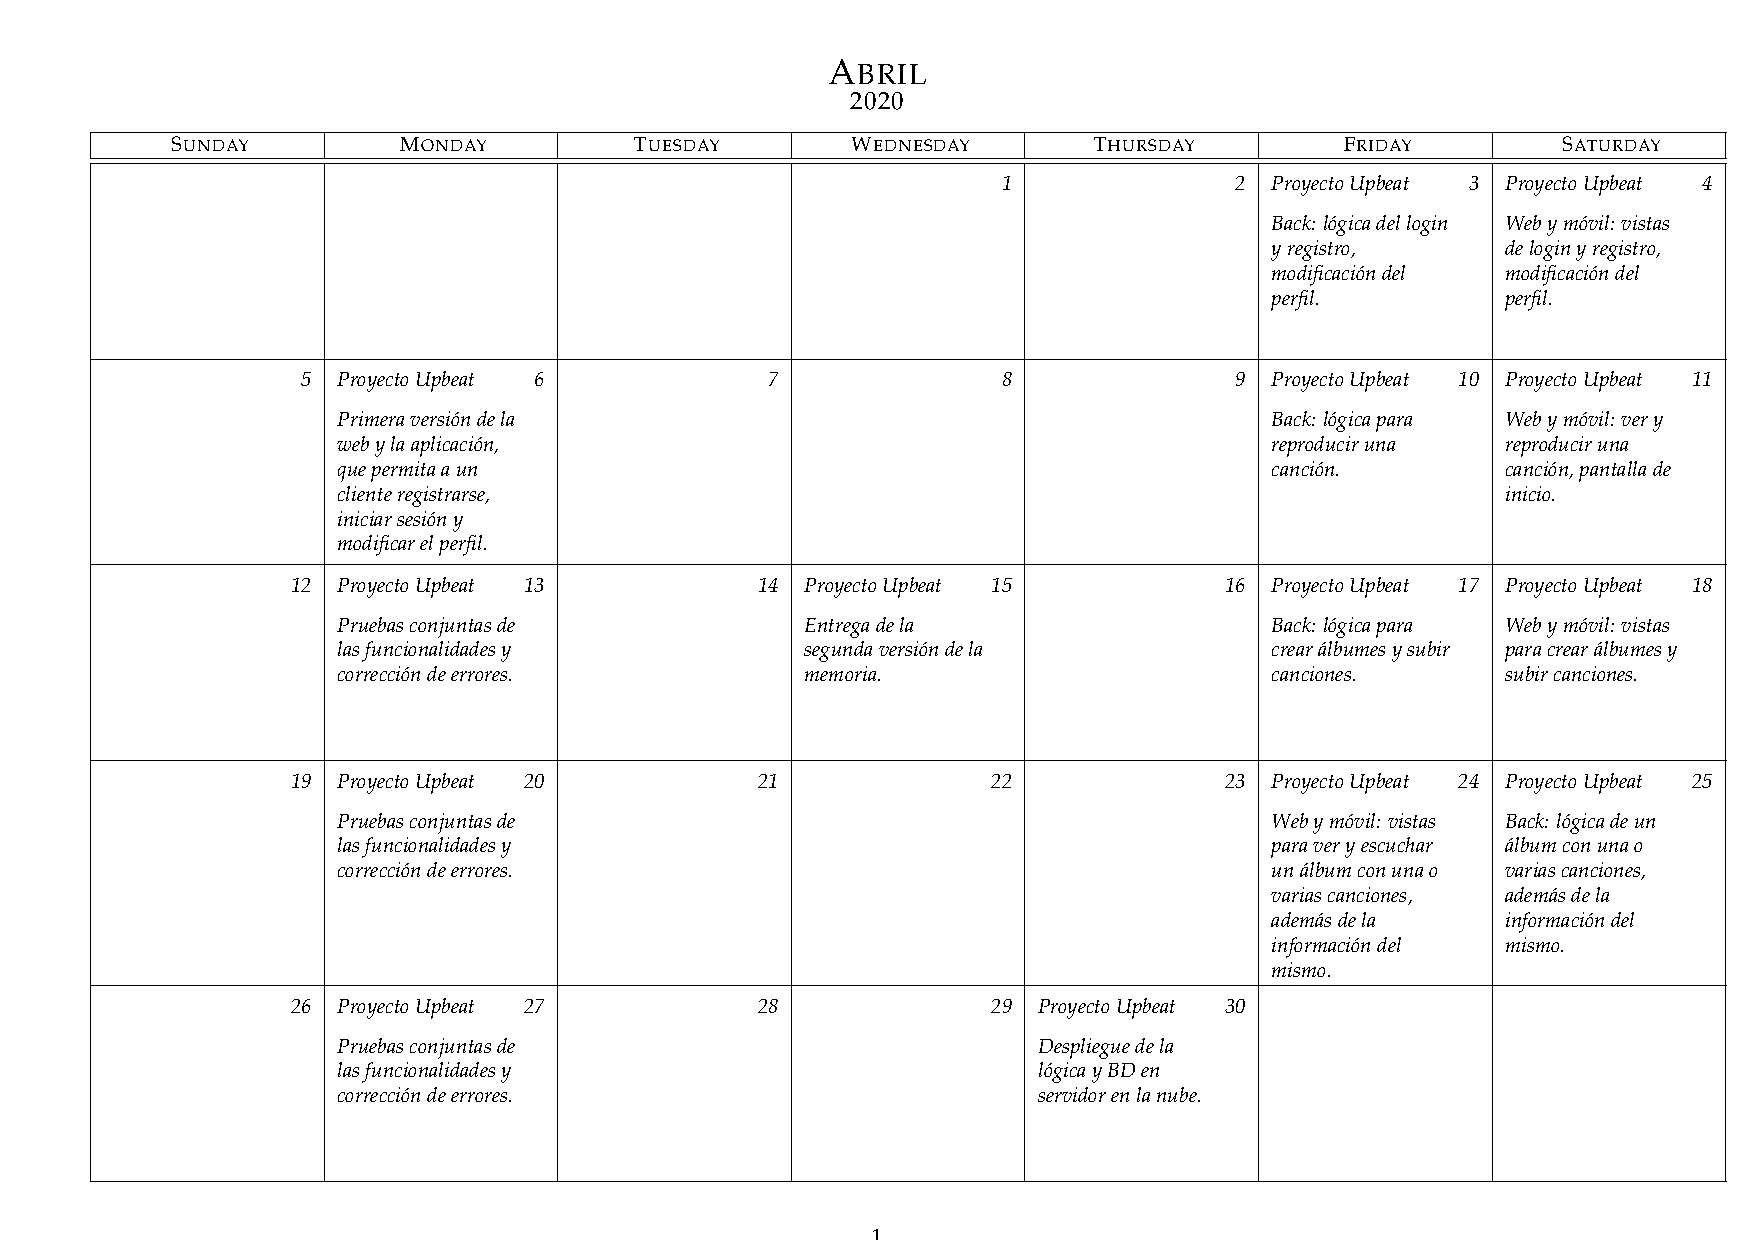
\includepdf[pages=1-2]{calendar.pdf}
\newpage

\subsubsection{Diagramas de Gantt de la aplicación}
\begin{figure}[H]
	\hspace*{-3.7cm}
	\centering{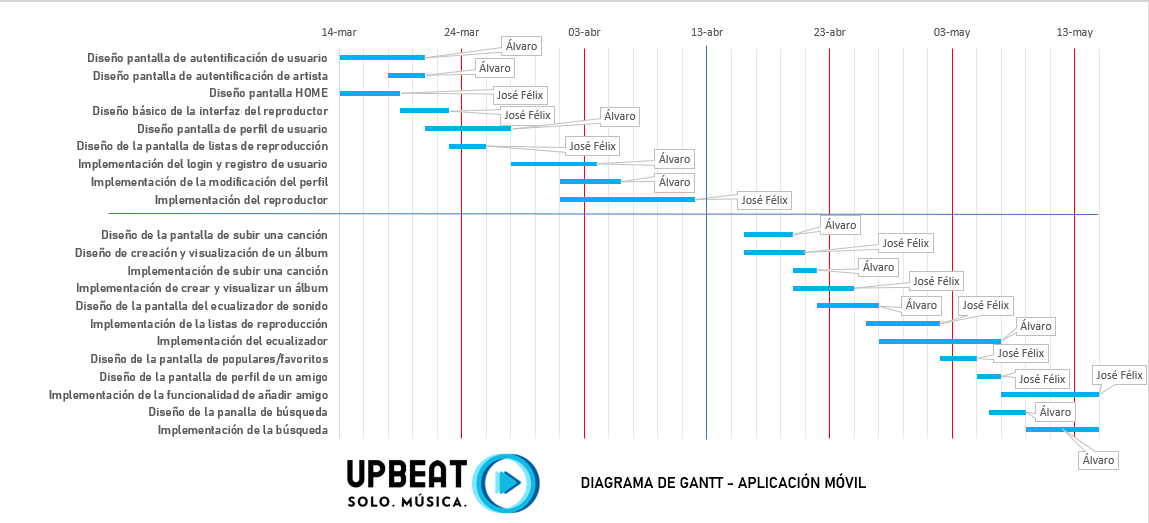
\includegraphics[scale=0.61]{Gantt_app.png}}
\end{figure}
\begin{figure}[H]
	\hspace*{-3.7cm}
	\centering{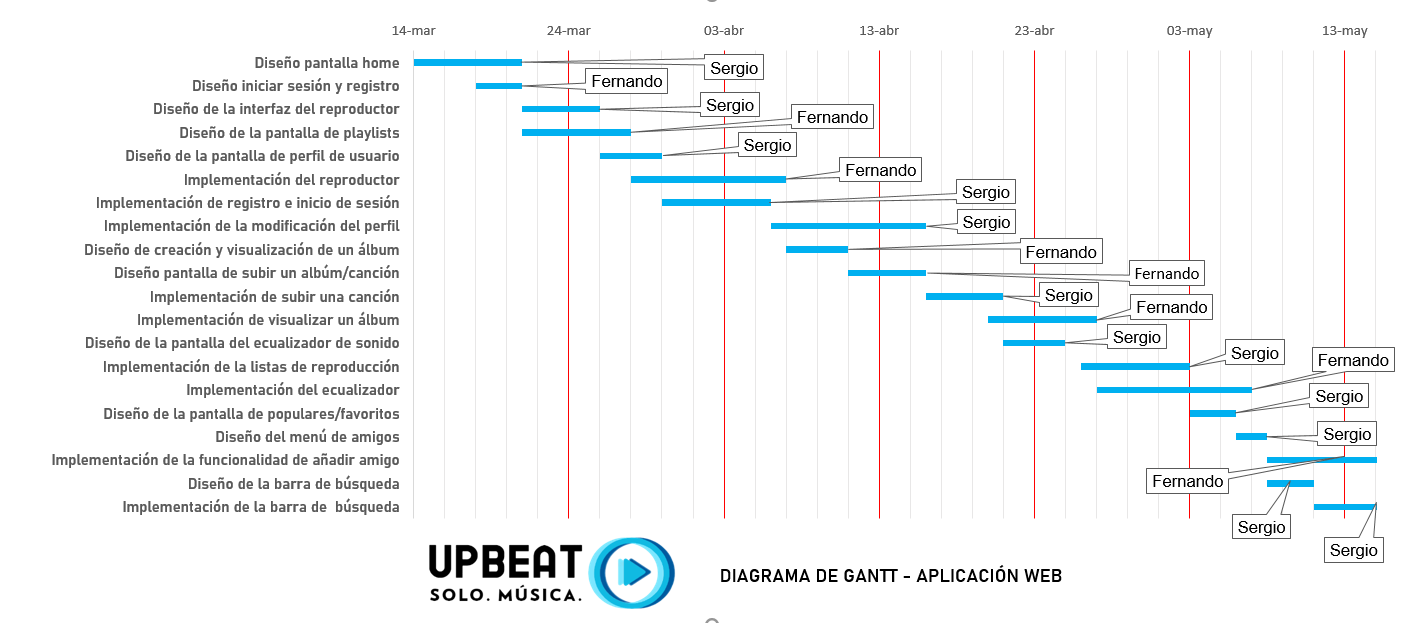
\includegraphics[scale=0.61]{Gantt_web.png}}
\end{figure}
\begin{figure}[H]
	\hspace*{-3.7cm}
	\centering{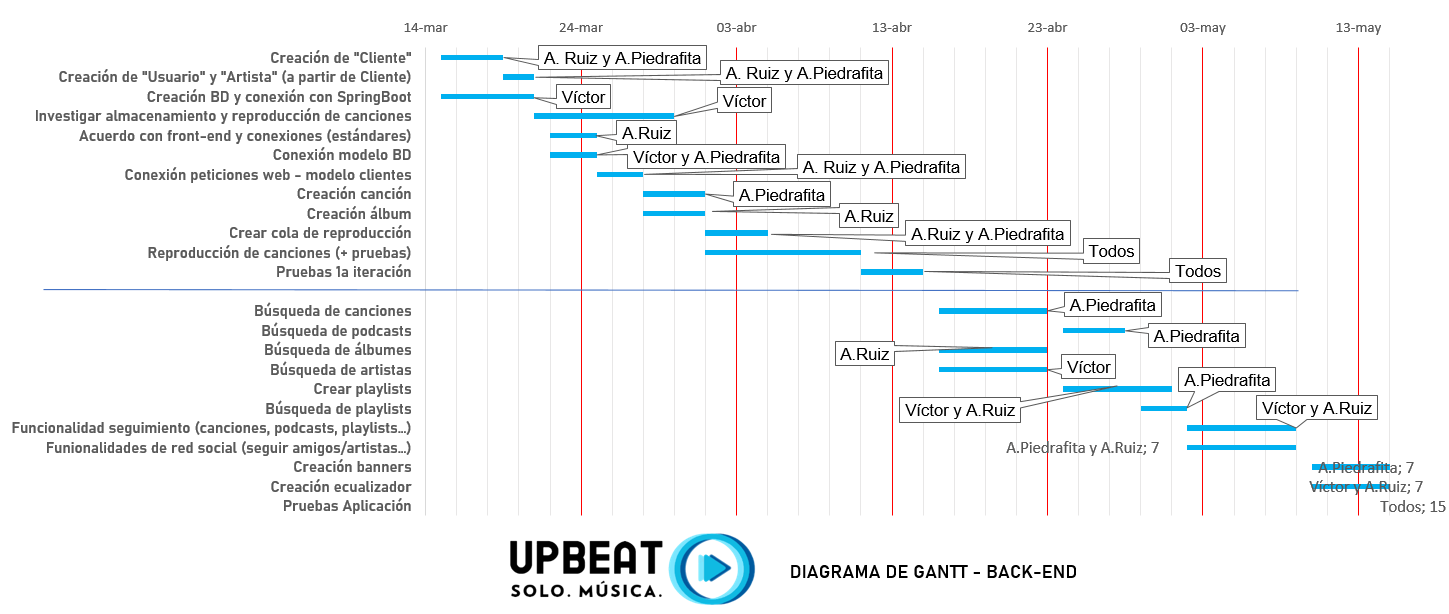
\includegraphics[scale=0.61]{Gantt_back.png}}
\end{figure}

\newpage
\section{Análisis y diseño del sistema}

\subsection{Análisis de requisitos}
Se exponen los siguientes requisitos funcionales de la aplicación:
\begin{table}[H]
	\begin{tabular}{p{4cm} p{10cm}}
		\hline
		\hline 
		\textbf{Requisito funcional}
		\vspace{0.5mm} & \textbf{Descripción} \\ 
		\hline
		\hline
		RF1
		& El sistema permite la existencia de clientes. \\ 
		\hline 
		RF2
		& Los clientes podrán ser usuarios normales o artistas. \\ 
		\hline
		RF3
		& Los clientes se registrarán mediante usuario y contraseña. \\ 
		\hline
		RF4
		& Un usuario es un cliente registrado que puede acceder a las funciones de la aplicación como escuchar canciones/podcasts, crear y seguir listas de reproducción, seguir a otros usuarios, escuchar álbumes y ver las canciones subidas por los artistas. \\ 
		\hline
		RF5
		& Un artista es un cliente registrado que puede realizar las mismas funciones que un usuario, además de crear álbumes y subir canciones. Crear un álbum consiste en la creación de un grupo de canciones que pertenecen al mismo artista. \\ 
		\hline
		RF6
		& Un cliente se compone de un nombre único, nombre personal y apellidos, un correo electrónico, una contraseña para acceder a la aplicación, una foto de perfil y las redes sociales que posee (si quiere añadirlas de forma opcional). \\ 
		\hline
		RF7
		& El sistema permite que los clientes modifiquen los datos de su perfil, es decir, su nombre, correo, contraseña, foto de perfil e información de las redes sociales. \\ 
		\hline
		RF8
		& Los clientes accederán a la aplicación mediante una aplicación móvil o una aplicación web. \\ 
		\hline
		RF9
		& El sistema permite reproducir y pausar una canción y/o podcasts. También permite saltar a la siguiente (si la hubiera), retroceder a la anterior, y elegir un bucle de la misma o reproducir aleatoriamente varias canciones y/o podcasts. \\ 
		\hline
		RF10
		& Una canción se compone de un título, un audio, artista/s que la han creado, género de la canción, país de la canción y veces que ha sido reproducida. \\ 
		\hline
		RF11
		& Una lista de reproducción es una lista de canciones generadas por un cliente. \\ 
		\hline
		RF12
		& El sistema permite que un cliente cree y borren listas de reproducción creados por ellos mismos, las cuales serán públicas. \\ 
		\hline
		RF13
		& El sistema permite que los clientes añadan canciones a las listas de reproducción creadas por ellos mismos. \\ 
		\hline
		RF14
		& El sistema permite que los clientes sigan listas de reproducción creadas por otros usuarios. \\ 
		\hline
		RF15
		& El sistema permite que solo los artistas puedan subir canciones. \\ 
		\hline
		RF16
		& El sistema permite buscar una determinada canción por nombre o género, además de un artista por nombre. \\ 
		\hline
	\end{tabular}
\end{table}
\break
\begin{table}[H]
	\begin{tabular}{p{4cm} p{10cm}}
		\hline
		\hline 
		\textbf{Requisito funcional}
		\vspace{0.5mm} & \textbf{Descripción} \\ 
		\hline
		\hline
		RF17
		& Las búsquedas por palabras clave deberán al menos contener una palabra, de mínimo cuatro caracteres. \\ 
		\hline 
		RF18
		& El sistema permite ver las canciones más populares de un país. \\ 
		\hline 
		RF19
		& El sistema permite ver las canciones más populares de un artista. \\ 
		\hline
		RF20
		& El sistema permitirá usar un equalizador al escuchar las canciones. \\ 
		\hline
		RF21
		& El sistema permitirá el uso de \textit{banners} para ofrecer publicidad. \\ 
		\hline
	\end{tabular}
\end{table}
Se exponen los siguientes requisitos no funcionales de la aplicación:

\begin{table}[H]
	\begin{tabular}{p{4cm} p{10cm}}
		\hline
		\hline 
		\textbf{Requisito no funcional} & \textbf{Descripción} \\ 
		\hline
		\hline
		RNF1 
		&  El sistema permitirá ser utilizar un diseño modular, un lenguaje fácil de entender, usar y mantener.\\ 
		\hline
		RNF2
		&  El cliente tendrá el desarrollo móvil en formato \textit{Android} e \textit{iOS}.\\ 
		\hline
		RNF3
		& El sistema permite almacenar canciones y podcasts en formato \textit{.mp3}, \textit{.WAV} y \textit{.OGG}. \\
	\end{tabular}
\end{table}
\newpage

\subsection{Diseño del sistema}
Un aspecto esencial que se ha considerado desde el principio ha sido la realización de la base de datos relacional en \textit{PostgreSQL}, siguiendo las siguientes razones:
\begin{itemize}
	\item Brinda opciones más complejas que otros gestores, ya que suele estar orientado para bases de datos más grandes y con consultas más largas. Algunas de sus funciones, como la de unir tablas, hacen que sea mejor valorado por algunos desarrolladores frente a su competencia.
	\item Código \textit{OpenSource}.
	\item Soporta todas las operaciones con \textit{Strings} como concatenar \textit{sub stringing}, búsqueda \textit{regex}, \textit{matching} y \textit{splitting}, búsqueda de texto completo y transformación de caracteres entre otros.
	\item Permite el uso de \textit{JSON} Y \textit{JSONB} en su totalidad, incluyendo varias funciones para el manejo de los mismos.
\end{itemize}
Fue elegido este gestor de datos porque, en comparación con los demás, permite de una manera simple almacenar los datos de las canciones, unido a una alta fiabilidad.
\newpage
El modelo \textit{Entidad - Relación} que se ha llevado a cabo ha sido el planteado a continuación, implementado en el back-end con esta estructura:
\begin{figure}[H]
	\hspace*{-3.9cm}
	\centering{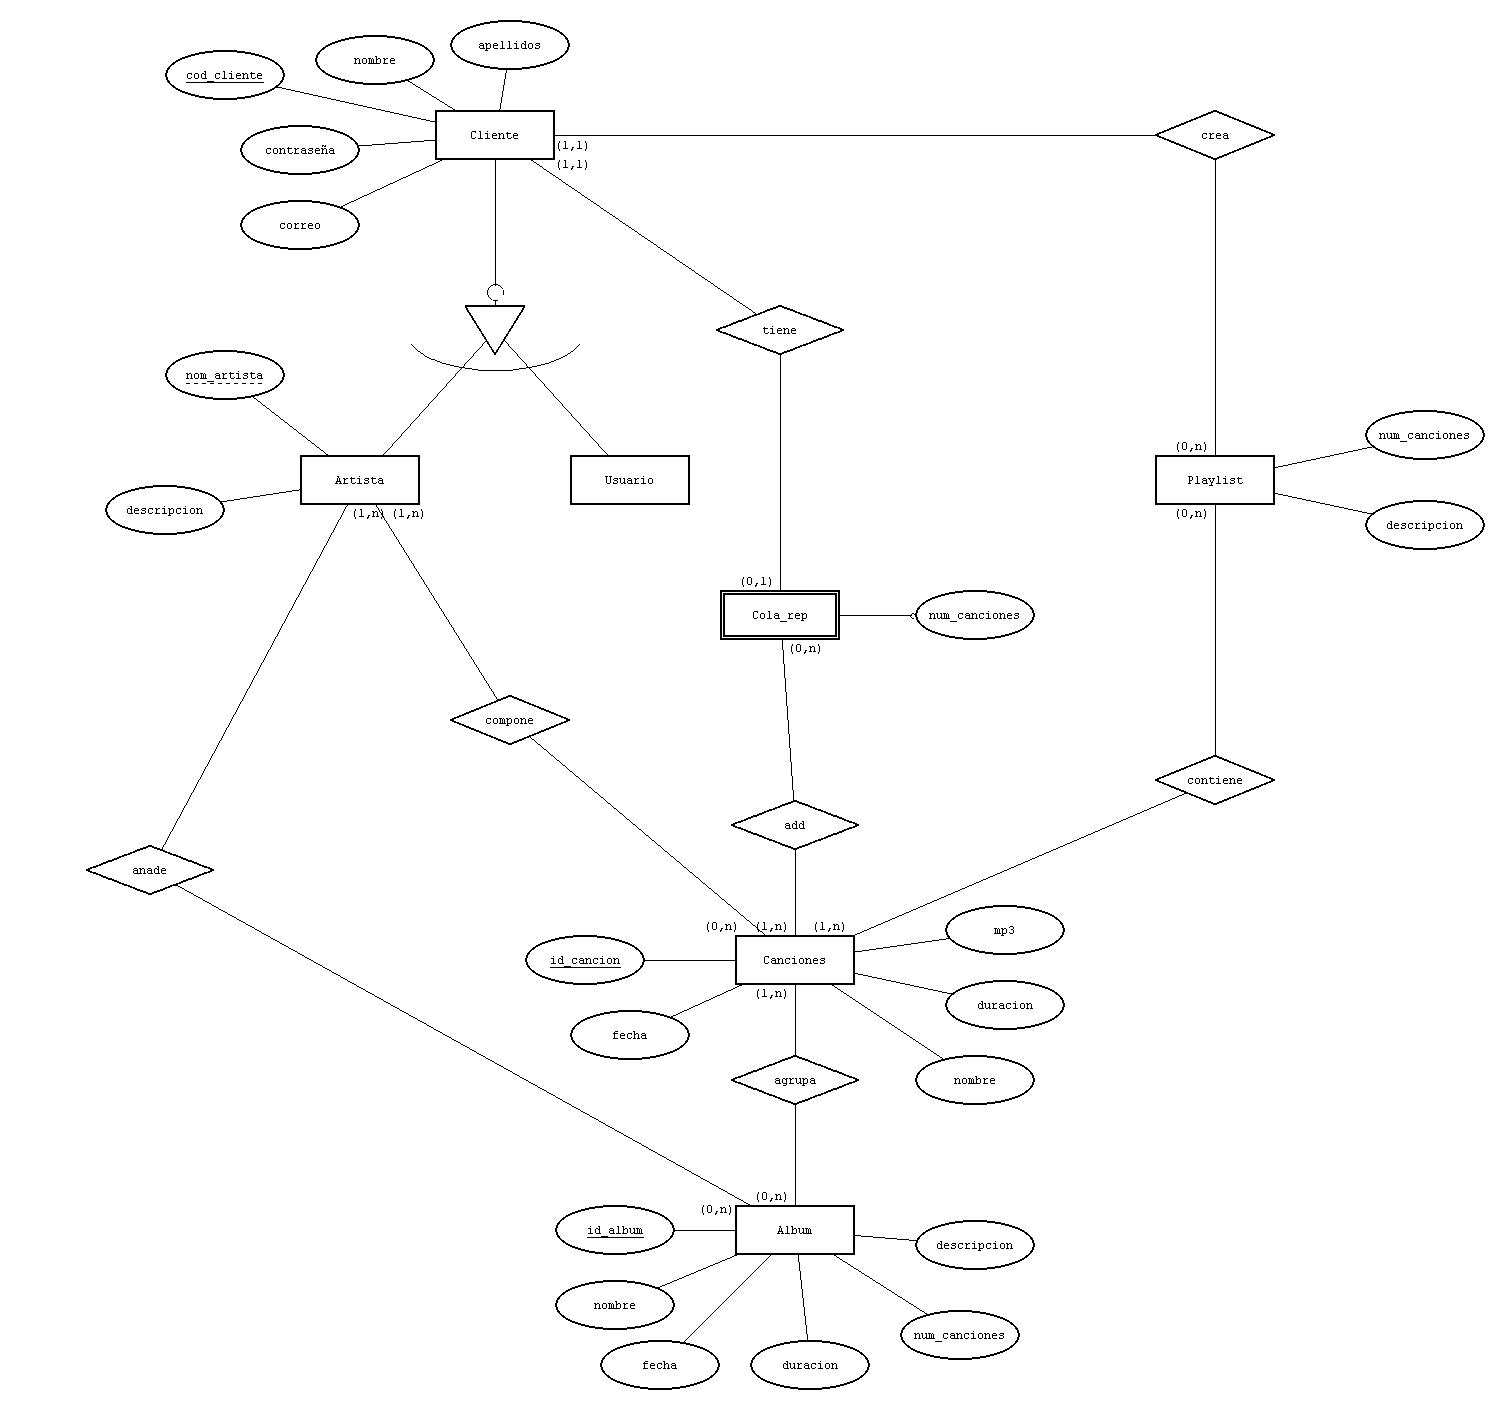
\includegraphics[scale=0.35]{ModeloER.jpg}}
\end{figure}
El diseño del back-end será \textit{REST} para todas las consultas y peticiones relacionadas con la aplicación, excepto la parte de las canciones en streaming. Para ello, se usará la siguiente tecnología CRUD: \textit{Spring Content(Cloud-Native Content Services for Spring)}. \\
\hfill \break
Esto es debido a que no hay que preocuparse de la implementación del código del controlador del reproductor para que soporte \textit{request} parciales (rangos de bits).\hfill \break
\textit{Spring Content} nos permite crear un servicio \textit{REST-based mp3}  que soporta streaming. Además, también aporta completamente la funcionalidad \textit{CRUD} (\textit{Create == POST}, \textit{Read == GET} (incluyendo rangos de bits), \textit{Update == PUT}, \textit{Delete == DELETE}) en caso de ser necesaria.
\begin{figure}[H]
	\centering{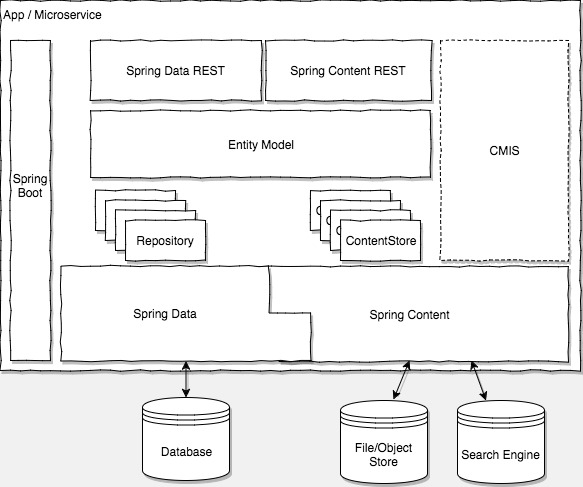
\includegraphics[scale=0.8]{upbeat_streaming.png}}
\end{figure}
\newpage
Por todo esto, la estructura del proyecto con la parte front-end incluida será lo siguiente:
\begin{figure}[H]
	\hspace*{-1.5cm}
	\centering{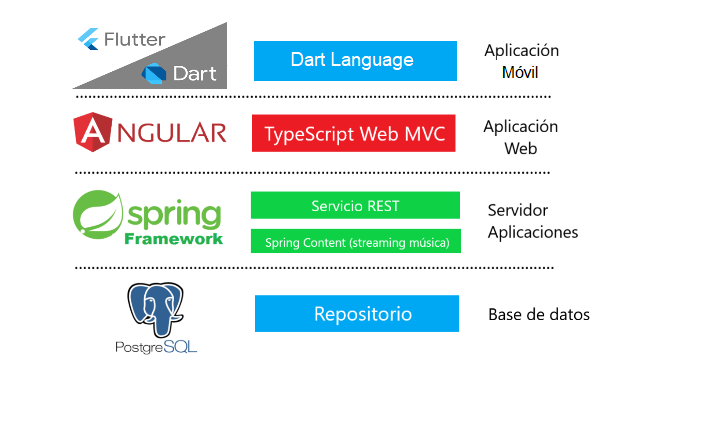
\includegraphics[scale=0.82]{EstructuraProyecto.png}}
\end{figure}
A la izquierda se denotan las tecnologías usadas para cada parte junto a la función que realiza cada una. \\
\newpage
La manera de comunicarse entre APIs sigue este patrón:
\begin{figure}[H]
	\hspace*{-2.5cm}
	\centering{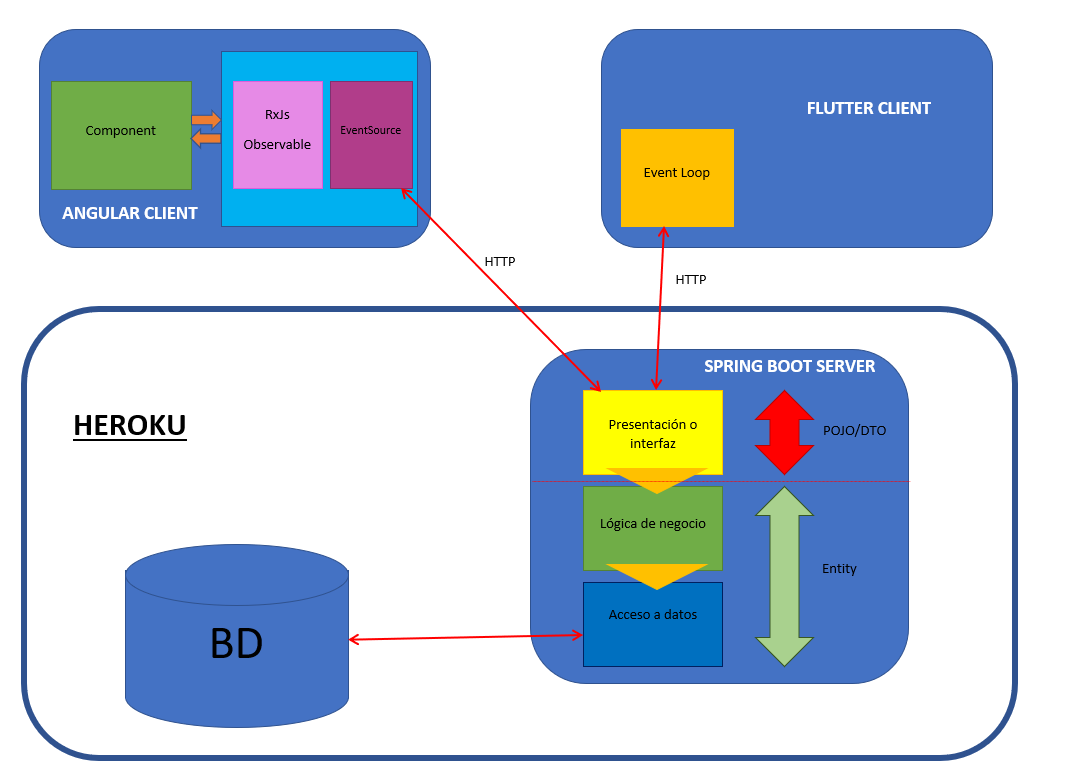
\includegraphics[scale=0.58]{EsquemaPS.png}}
\end{figure}
\section{Memoria del proyecto}
\subsection{Inicio del proyecto}
Al principio del proyecto, se creó el documento de propuesta técnica y económica. Este documento está disponible en la carpeta Memoria del \textit{GitHub} del proyecto, donde se explica con más detalle.\\
Una vez creado, se asignaron roles a los distintos integrantes debido a que se trata de un proyecto complejo. Los roles como ya se han mencionado, corresponden con: el jefe del proyecto cuya función principal es la organización, reparto y optimización del trabajo, así como la resolución de posibles disputas en el grupo. 
Se encarga, además, de verificar que todas las tareas sean realizadas a tiempo. \\
\hfill \break
Otro rol sería los responsables de la redacción de las actas, redacción de los documentos no técnicos y por último, los encargados de la redacción de los documentos técnicos y despliegue. Otro rol asignado era la redacción de los guiones de reunión, realizados cada vez que se comunicaba con el profesor. Otros roles, por ejemplo, serán los encargados en la base de datos y servidor, realizando todo el mantenimiento y creación. Similares roles referentes a la aplicación se pueden dividir en 2, los encargados en el diseño de la interfaz web y los encargados en el desarrollo de la interfaz móvil. \\
\hfill \break
El desarrollo del proyecto se realiza a través de la plataforma \textit{GitHub}, de forma que todos los componentes del equipo desarrollan parte del software, y lo ponen en común en dicha plataforma. Se establecieron varias carpetas para cada una de las funcionalidades de la aplicación. \\
Por último, para la elección de las tecnologías usadas, se tuvo principalmente en cuenta los conocimientos del equipo de desarrollo, ya que cuanta mayor experiencia tuviera menos horas aprendiendo dedicarían. Las tecnologías elegidas fueron: bases de datos \textit{SQL}; lenguaje \textit{Dart} para la aplicación móvil; \textit{Angular}, \textit{CSS}, \textit{JavaScript} para web.
\subsection{Ejecución y control del proyecto}
El equipo de \textit{Flutter} ha divido el trabajo hecho hasta ahora en dos partes. Álvaro se ha dedicado a realizar la parte de registro y login de usuarios, mientras que José Félix se ha dedicado a hacer las pantallas de canciones, playlists, álbumes y podcasts. La comunicación dentro del equipo se ha realizado a través de los mensajes privados de \textit{Whatsapp} ya que solo cuenta con 2 integrantes.\\
\hfill \break
Para controlar el trabajo realizado se ha utilizado el \textit{Issue Tracker} de \textit{GitHub}, aunque también nos hemos comunicado por \textit{WhatsApp} para tener una comunicación más activa.
A día de hoy, vamos algo por detrás del plan inicial ya que no esta implementado el reproductor con la base de datos, solo se ha implementado por ahora la parte front-end sin funcionalidad. Esto es debido a que la parte del back-end de las canciones aún no esta con funcionalidad completa.\\
\hfill \break
No se ha producido ningún cambio en las tecnologías empleadas.
No se han producido problemas con las integraciones ni versiones del código.
Por ahora las únicas pruebas realizadas han sido comprobar que el front-end se comunica correctamente con el back-end, realizando las consultas e inserciones en la base correctamente.\\
\hfill \break
En la parte del front-end web se ha tenido que cambiar la distribución de trabajo, informándonos simultáneamente la mayor parte del tiempo porque no teníamos experiencia previa y había errores de conexión con el back-end que se sabía solventar; todo esto ha llevado mucho tiempo entre leer documentación y realización de pruebas. También cabe reconocer que si se hubiera puesto en contacto antes con los miembros del back-end se habría solventado mucho antes porque eran errores mínimos.\\
\hfill \break
En lo que respecta al back-end, se ha trabajado principalmente por videollamada, trabajando sobre el mismo o diferentes temas, pero cooperando y preguntando dudas en caso de que algún miembro se quede atascado. Previo a esto, han sido necesarias varias horas de formación ya que en la mayoría de los casos no se conocían ni la forma ni el entorno de trabajo. 
Este factor ha hecho que este trabajo haya supuesto un esfuerzo mayor del que podría haber requerido realmente con respecto a las horas.
Además, se intentado y se ha conseguido desplegar la aplicación en la plataforma \textit{Heroku} para que, cuando se produzca un commit desde la rama master, se suba automáticamente el proyecto y todos los miembros (también desde el front-end) puedan hacer peticiones a las \textit{URLs} previamente acordadas.
\subsection{Cierre del proyecto}
Los tiempos en las estimaciones iniciales han sido ligeramente más cortos que los utilizados realmente, ya que aunque también estemos utilizando el mismo lenguaje en la asignatura de Arquitectura Software ninguno de los dos lo habíamos utilizado anteriormente.\\
\hfill \break
Las lecciones aprendidas más importantes han sido tanto, tanto aprender como utilizar \textit{Flutter} y programar en \textit{Dart}. Además, hemos adquirido conocimientos sobre cómo funcionan las cabeceras \textit{HTTP} para poder hacer peticiones al back.\\
Como se ha indicado anteriormente Álvaro se ha dedicado a hacer la parte de registro y login de usuarios, llevándole unas 16 horas, y José Félix ha hecho las pantallas de canciones, playlists, álbumes y podcast, con un total de 12 horas.\\
\hfill \break
En el front-end web se tiene en cuenta un pequeño retraso enfocado en el diseño de algunos módulos de la web, pero en estas semanas se espera solventar y ponerse al día con el calendario establecido al principio. De igual manera, se supone que las variaciones serían mínimas. Junto a todo esto, el proyecto ha supuesto bastante esfuerzo al principio, y muchas horas de documentación y tutoriales porque no se poseía experiencia suficiente con Angular.\\
\hfill \break
Por último, en la parte del back-end, se ha completado la parte del registro e inicio de sesión de los usuarios, se ha conseguido desplegar automáticamente y poder estar accesible para todos los miembros el proyecto, y se ha investigado y se está probando el almacenamiento y la reproducción de canciones, así como el almacenamiento de imágenes. La correspondencia con el calendario no es exacta, ya que se ha priorizado el despliegue para una mayor comodidad de todos los miembros del equipo pero no se ha completado aún (aunque está en proceso) como se había definido previamente el almacenamiento y la reproducción de las canciones.
\end{document}


